% !Mode:: "TeX:UTF-8" 

\BiChapter{文本立场分析相关研究}{Methods of inserting figures}

本章概要介绍立场分析及其相关研究。首先从目前研究相对成熟的文本情感分析入手,分别从传统的基于规则、机器学习、深度学习分别讨论文本情感分析技术。作为本文的重点研究对象详细介绍了分别基于机器学习和深度学习模型的文本立场分析技术相关研究 本章总结了各项研究工作的特点,在分析优缺点的基础上引出本文的后续研究

本章2.1节介绍了文本情感分析的相关研究,2.2节介绍了文本立场分析的相关研究。


\BiSection{文本情感分析相关研究}{2.1}
文本情感分析,指应用自然语言处理、文本分析、计算机语言学等技术系统的定位、提取、量化文本信息中作者所有表达的个人主观信息。文本的情感分析是自然语音处理的重要研究内容之一,且其具有重要的科研价值与商业实用价值,吸引了大量的研究人员的关注。研究人员从不同的角度和不同方法对文本情感分析展开了研究。本节将从基于情感词典、机器学习和深度学习的三个方向分别概述近年来情感分析的研究进展。


\BiSubsection{基于情感词典的文本情感分析}{2.2.1}
基于情感词典的文本情感分析是早期研究人员的成果,其相应的模型建立在情感词典和语言学的规则基础上。由于模型的解释性好,需要计算资源较少,成为早期研究文本情感分析的主流。情感词典作为文本情感分析的重要组成部分能给文本情感分析提供重要的特征信息。情感词典的构造通常由语言学领域的专家完成。例如现有相对成熟的情感词典有WordNet、HowNet、大连理工大学中文情感词汇文本库等。基于情感词典的文本情感分析的技术步骤通常先匹配原文本中与情感词典相对应的情感表达特征词,然后根据各特征词的表达方式综合计算其每一个特征词的情感得分,最后结合整个文本的情感得分总结文本的情感倾向。

针对中文评论中情感分析问题,姚天昉\citeup{yao2017}提出一种基于句法依存关系与领域本体来分析评论情感的方法,此方法首先建立相应的推导规则,然后通过句法依存来定位与分析谓语的情感倾向,通过已设定的规则将谓语所具备的情感倾向传递给相应的主题词与宾语。Taboada\citeup{taboada2011lexicon}在原来情感词典的基础上进一步考虑了词语的词性,结合情感词和词性综合给出情感的倾向得分。该情感分析模型包含一个语义指向计算器,这个计算器首先抽取出文本中的形容词、动词、名词以及副词等情感方位词,然后结合各种情感方位词计算原来文本的情感指向,模型结合的情感指向和强调、弱化、否定等转移的价位得到文本最终的情感倾向。作者通过一系列的实验证明了基于情感词典和此种转移规则的模型具有很强的鲁棒性,在跨领域的的文本情感分析上也有良好的表现。孙建旺\citeup{孙建旺2014基于词典与机器学习的中文微博情感分析研究}等提出结合情感词典和机器学习两者的优势来解决微博情感分析的问题利用微博多层次结构对微博文本进行特征降维。此外,由于微博包含多种颜文字,表情符等特点,设计了对颜文字和表情符的情感计算方法,其实验证明了加入表情符等特征,对微博的情感分析效果得到了提高。

基于不同的上下文可能决定某些情感词的特点,具有一定的领域相关性。例如“高”在“质量高”的上下文中表达的是正面的情感倾向,但是如果在“消费高”的上下文则表达负面的情感倾向。Bollegala\citeup{bollegala2013cross}等人结合了不同领域对情感词的表达特点构造了领域相关的情感词典。实验证明结合领域知识的情感词典能在相对于的领域取得更好的效果。Li\citeup{li2012cross}提出一种相关领域自适应情感词的框架,能同步从标注训练语料中提取出的主题词和情感词,并进一步通过分析标注语料中主题词和情感词的关系来推导出未标注语料中与主题相关的情感词。

总体来看,基于情感词典/规则和知识库的情感分类准确率较高,但由于情感词典和常识库规模的限制,覆盖率较低。同时此类方法对分词、词性标注、规则匹配等的准确性要求较高,系统内部错误传递影响较大。

\BiSubsection{基于机器学习的文本情感分析}{2.2.2}

随着机器学习成功应用于其他领域的快速发展,对于文本情感分析的问题,大量的研究人员开始开展基于机器学习的文本情感分析的研究。基于机器学习的文本情感分析方法,首先通过特征工程抽取文本情感分析特征,然后通过抽取出来的特征词用机器学习能理解的数值表达文本。通过人工标注建立起特征表示数据和情感类标对的训练数据,通过各种已有的机器学习模型提取出训练集中特征和类标之间的映射关系的模型。Pang\citeup{pang2004sentimental}等研究人员创新性的把文本主题分析的技术迁移应用到文本情感分析中,文本的主题分析主要根据与主题相关的主题词决定,但是表达情感的方式更加的多样化,需要考虑的因素则更多。Pang把文本的情感分析看成一类特殊的主题分析,使用了在有监督学习上泛化能力较好的支持向量机、朴素贝叶斯、最大熵模型三种基础的分类模型。选用的分类特征为一元词组(Unigram)、二元词组(Bigram)、词性分析(POS)、形容词位置信息等。此研究通过组合特征和模型的交叉验证表明,三个分类器组合任意一个特征的性能都比基线模型要好,在有关电影影评的数据集上,一元词组(Unigram)结合支持向量机的模型取得了良好的效果。但是此研究实验也论证了文本的情感分析的性能还是和文本主题分析存在较大的差距,同时也佐证了文本情感分析对模型和特征也有更高的要求。

为了减少文本中无关的客观信息对文本情绪分析的干扰作用,Pang和lee对上述基于机器学习的文本情感分析模型进行了有针对性的改进,规避了文本客观消息的干扰,使模型更加专注于文本的主观信息。作者他们把原来的文本情感分析问题转换成以各字句连接图中最小割问题,应用了挖掘图中的最小割的分类器来寻找对情感分析有用的主观表达的句子,从而屏蔽掉客观消息的干扰。此研究的实验也论证了剔除客观信息的文本情感分析模型的性能得到显著的加强。

Xiang\citeup{Xiang2014Improving}等研究人员在社交媒体文本中进一步研究文本情感分析,针对Twitter文本情感分析任务中只考虑表情符、一元词组和句法分析等局部特征信息的问题,提出一个考虑全局主题信息的方法。此方法首先利用支持向量机分类器提取通用情感分析特征,然后在原模型基础上进一步考虑主题信息。实验证明这种融合主题与情感信息的模型在英文数据集上具有较好的性能,证明融合主题与情感信息方法的有效性

\BiSubsection{基于深度学习的文本情感分析}{2.2.3}

深度学习由于其更复杂的模型和更多的参数,比起以往的的机器学习方法在海量数据集上更有优势。且深度学习具有能够以端到端的形式构建模型的优势,不再需要人工筛选特征,所以近来得到研究人员的关注。Socher\citeup{socher2010learning}等研究人员建立了影评情感树状数据集,数据集包含了11,855条有关多个电影的影评句子,这些句子又可分成215,154个不同短语。其中任意短语构成的节点和其他叶子节点均被标注为五类情感(强正面、正面、中性、负面、强负面)中的一个。作者应用语法树和词汇向量代表了不定长的短语来构建循环神经网络,因此通过此模型可获取句子中所有短语的具体情感表示向量。作者提出的树形结构能很好的感知各短语情感之间的变化和定位否定作用具体范围,同时也能有效的定位情感表达中转折表达。通过具体的实验表明RNTN网络在五分类(强正面、正面、中性、负面、强负面)和二分类(“正”、“负”)的情感分析任务中均获得最佳效果。

在基于深度学习的文本情感分析任务中,低维稠密的词向量对最终深度学习模型的性能有者巨大的影响。Mikolov\citeup{mikolov2013efficient}提出Word2Vec模型能从大量的无监督语料中有效的学习固定长度词向量表示,但是这种建模只考虑到了上下文位置的信息,遗弃了词语本身所包含的情感信息。例如英文中的“good”与“bad”具有大量相似的上下文,若只采取Mikolov所提出的Word2Vec模型,两者将拥有相似的词向量,但是对于文本情感分析任务,两者包含的情感信息存在巨大的差异。针对Word2Vec在文本情感分析词向量预训练存在不合理性,Tang\citeup{Tang2014Learning}在原来词向量训练的基础上增加对句子的情感分类,此研究在微博语料中进行实验。通过不同的表情符号在大量无监督微博文本中删选出“正向”与“反向”情感的微博,在词向量的预训练后建立二分类网络结构来判定微博情感的倾向。使得词向量在包含上下文信息的基础上添加情感倾向。在SemEval2013情感分析数据集实验效果表明使用情感词嵌入的情感分类模型的有效性。

Cao\citeup{Cao2015Combining}针对卷积神经网络在处理文本情感分析非线性问题处理效果不佳的问题,提出一种结合卷积神经网络与支持向量机的文本情感分析方法,首先作者利用CBOW模型在大规模无标注数据中预训练词的低纬度稠密的词向量表示,然后通过多窗口长度卷积神经网络学习每个句子的向量表示,学习后的句子表示作为支持向量机的特征输入。模型中卷积神经网络作为特征学习器,支持向量机代替原有全连接分类层。融合后的模型在NLPCC2014情感分析中英文数据集上均超过了测评的最佳系统,实验表明所提结合深度学习与支持向量机方法的有效性。


\BiSection{文本立场分析相关研究}{2.3}
文本立场分析与文本情感分析有着本质的区别,文本立场分析更加关注文本反应出作者对于某一特定主题目标所持的立场和倾向。立场分析需要结合主题目标和情感信息,这比单独考虑文本的消息更加具有有挑战,对模型的建模能力也有更高的要求。作为一项特殊的情感分析任务,立场分析问题主要是在给定了目标的前提下,判断这个文本的立场是“支持”或“反对”。作者在文本中评价的目标不一定是立场分析给定的目标,也可能立场分析给定的目标并没有直接出现在文本中。即使作者在文本中对目标/实体的态度是积极的,但推断出来的结果可能是作者对给定目标持反对的立场。本节将分别介绍基于机器学习与基于深度学习模型的文本立场分析研究状况。


\BiSubsection{基于机器学习的文本立场分析}{2.3.1}

基于有监督学习的机器学习方法广泛应用于文本立场分析任务中,Somasundaran\citeup{Somasundaran2010Recognizing}等建立一个论据触发词词典,词典用于检测定位论据、情感表达与目标相关信息,这些信息用于作为后续有监督学习分类器的特征。Anand\citeup{anand2011cats}抽取了网络中论坛上4837篇有关多个不同话题的讨论,构造了10种不同的特征。这10种特征包括一元词频、二元词频、长度、标点、线索词、句法依赖、语义依赖、广义依赖、上下文特征和等。分别利用RIPPER和朴素贝叶斯两种算法验证了立场分析在不同特征集合下的效果。实验证明,应用了上下文特征可以有效提升实验效果,在不同子话题中模型效果表现出较大差异。Walker\citeup{Walker2013Stance}在Anand原有特征基础上进一步讨论了支持与反对对话的结构信息。针对Anand忽略了文本间意识形态和用户交互这两种对实验性能具有很大影响的约束。Hasan\citeup{hasan2013stance}在研究中的文本序列模型是以相邻文本间的用户交互约束建立的,并利用了条件随机场来解决序列标注问题。该研究为每位文本作者的意识形态以ILP建立基于话题领域、作者的意识形态约束模型。并且在实验中得到了提升。

社交文本以推特为例,具有长度较短且语言非正式等特点,Zhang\citeup{zhang2016ecnu}针对这些特点提出了两部的学习系统。将社交媒体文本的三个立场“支持”、“反对”和“其他”转化为两次两分类的任务。第一步进行文本相关性检测,可以将无关文本作为“其他”类型检测出来;第二步使用立场倾向检测模型,对文本进行“支持”“反对”二分类。该研究在传统语言特征外还应用了LDA(Latent Dirichlet Allocation)生成的话题相关性、主题只是、情感词汇、词嵌入和表情符等多种不同的特征组合,为每一组子话题数据分别使用线性回归模型(Linear Regression,LR)简历立场分析模型。并且考虑到不同话题数据分布具有差异,对这来年各个子模型验证了不同超参数和特征集的组合方式。最后用实验证明了对不同子任务和子话题使用不同的特征组合的方式是有效的。

除了不同特征组合可以起到提升立场分类效果的作用,构建具有差异性的分类器组合也同样可以提高模型的立场分类性能和泛化能力。Xu等\citeup{xu2016ensemble}提出了选取了Document2Vec、浅层语义分析、主题模型等特征。在随机森林、线性支持向量机和迭代集成分类器等多种分类器中测试性能,Xu采用了对基分类器线性组合的方式提升模型表现,具体如公式~\ref{a23333}~所示。
\begin{equation}\label{a23333}
p(C|x)=\sum_{i=1}^m w_i \cdot p_i(C|x)
\end{equation}

式中$p_i(C|x)$为文本$x$在第$i$个分类器中被预测成立场类别$C$的概率。

$w_i$为线性模型中及分类器第$i$个基分类器的权重。

$p(C|x)$为文本$x$在立场类别$C$中的概率。

实验证明,该模型可以提高文本立场分析的性能与泛化能力。

弱监督学习是一种基于噪声训练数据的半监督学习方式。不同于以往基于可靠训练数据的有监督学习方式,弱监督学习基于的是不严密的假设生成训练数据。在训练数据中更可能含有错误和大量噪声。但该方法可以避免人工标注的高昂成本,且能在新语料、新话题中具有较好适用性。

Ebrahimi\citeup{ebrahimi2016weakly}提出了使用关系自扩展来实现弱监督学习的立场分类法扩展种子训练集。定义了三种立场相关约束:相似文本表达的立场相似、具有朋友关系的作者立场相似和文本作者对话题的立场相似。Ebrabimi为了匹配含噪音的少量标注集合,首先使用若干短语模式,然后利用基于统计关系学习的合页马尔科夫随机域模型标注文本立场,最后使用结合词典、多元词组和情感类型为特征的线性核SVMs训练有监督的立场检测模型,并在SemEval英文立场分析数据集上具有较高的性能。

Dias\citeup{dias2016heuristics}提出了使用启发式规则的方法自动标注Twitter文本,可以解决弱监督学习中语料标注的问题。该方法可以达到两重目的,既可以使用监督学习算法自动创建训练语料库开发预测模型,又可以补充预测立场检测模型。Dias构建了7条启发式规则构建训练语料,分析了六个不同的立场分析任务,取得了可观的成果,加权F1值从52\%提升到了67\%。

Moharmmad\citeup{mohammadstance}提出了一个同时包含对特定主题目标的立场和句子情感极性的数据集,探讨了情感分析与立场分析的关系。作者提出一种以字符级别的N元词频、词级别的N元词频、迁移学习来的情感极性和词的分布式表示等作为特征的线性SVM分类器的方法。虽然提出模型较为简单,但在数据集上的表现超过已有的评测模型。通过多组对比实验表明情感极性分析结果对立场分析的效果有限。作者指出人类能轻易对不同主题目标做立场分析,而自动标注系统在这种不同主题目标情况下的性能则不是很理想。


\BiSubsection{基于深度学习的文本立场分析}{2.4}

近年来深度学习不仅在计算机视觉、语音识别等领域取得了卓越的成果,在自然语言处理领域中研究人员开始采用深度学习模型。不同于传统机器学习方法的手动特征工程,深度学习模型采用端到端的分类模式,减少人为手工构造特征的工作量,能够自动抽取在参数学习中最优的特征表示。本节介绍深度学习模型在立场分析方法上的应用。

\begin{figure}[htbp]
	\centering
	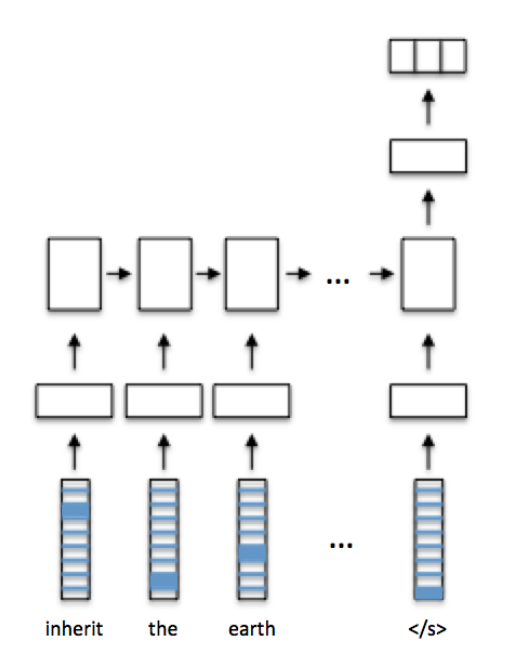
\includegraphics[width = 0.5\textwidth]{transfer_learning.png}
	\caption[rnn_vanish]{基于主题标签信息迁移学习模型}
	\label{chart_nlpcc_best_model}
\end{figure}
Zarrella等\citeup{zarrella2016mitre}研究人员利用了迁移学习的思想,首先利用word2vec等无监督方法训练了单词和短语的词向量表示。采集了大量的无标注Twitter文本。选取了词频高于100的词汇,然后用Word2vec模型预训练好了每一个词的256维度的词向量,后面通过词向量相似度选取比较关键的以\#为前缀主题标签,通过训练神经网络预测主题标签。后通过迁移学习的思想对网络结构进行微调来达到立场分析的目的然后通过主题标签预测辅助任务来学习句子向量,然后被微调用于标记样本的立场检测。实验结果显示,该方法在Semeval2016英文立场分析数据集任务中微平均F1值为0.678。

Yu\citeup{yu2016stance}提出了基于双向LSTM-RNN的模型,此模型包括词嵌入输入层、卷积层、池化层、LSTM单元层、全连接分类层。卷积层的作用是在于提取词组中的局部特征,LSTM单元的作用是学习句子的全局语义特征,池化层的作用是保留卷积的位置不变性和较少模型参数。组合上述的句子特征表示连接全连接层进行分类。实验证明模型在NLPCC中文立场分析数据集具有较好的性能。

Wei\citeup{wei2016pkudblab}等利用多卷积核文本CNN的模型处理Twitter立场分析任务,Wei所建立的网络包含词向量嵌入层、多核卷基层、最大化池化层与全连接分类层。其中文本的卷积窗口程度为3、4和5,每一个窗口长度包含100个不同的卷积核,采用ReLu函数作为激活函数。为提高模型的稳定性,Wei利用五折交叉验证的分割原数据集为不重叠的平行数据集合,并采用特殊的投票方式来决定Twitter最后的立场。模型在Semeval2016英文立场分析数据集TaskA取得第二的成绩。Wei为了解决在弱监督立场分析中标注数据缺失的问题,使用了分成两步任务的框架。首先构建一个基础的二分类器,使用他们定义的softmax层在二分类训练数据中执行三分类任务。第一步利用有清晰倾向性的词汇和表情标注“支持”和“反对”两种立场,第二步将“支持”立场和“反对”立场概率差绝对值小于阈值的文本标注为第三类“中立”。以弱监督标注文本为基础,使用与有监督学习相似的深度学习模型得到的预测结果的方法改善了训练数据较少的问题。

Sobhani\citeup{Sobhani2017A}建立了一个多目标立场分析数据集,此数据集包含一共包含4455条有关美国大选的Twitter文本。多目标数据集中包含Clinton-Sanders,Clinton-Trump和Cruz-Trump三对双目标文本。其中每一条Twiiter数据包含对2个目标的立场。作者也直接在多目标数据集中划分出了训练集、测试集和验证集。作者在多目标数据集上实验了多种神经网络模型,实验结果论证了把目标相关的数据联合训练的效果要优于直接单独训练每个目标的模型。在相关目标的数据中,有大量的共同模型可以利用来提高联合学习的性能。作者同时也提出一种把多目标联合学习的模型转换成类似于神经翻译模型的序列到序列模型,模型包含编码与解码两个过程。由于当前目标立场标签的生成条件相关于上一个目标立场标签,因此模型移除了不同目标之间的立场是相互独立的假设。作者对比了独立SVM、窗口滑动SVM、串联级别SVM与序列到序列模型在多目标立场分析数据集的性能,实验结果显示了相关目标联合学习的序列到序列模型的有效性。





\BiSection{本章小节}{2.5}

本章首先介绍了情感分析的常用技术和研究现状,然后从基于特征工程的机器学习方法和端到端的深度学习模型详细描述了立场分析检测的现有研究。基于特征筛选和分类器集成学习仍然是机器学习领域的主流,基于端到端的RNN和CNNs等模型的工作是在深度学习领域上的主要方案。特有的预置话题包在分析任务任务中对最后的预测也起到了十分关键的作用,立场分析现有工作的重要方向就是如何更好的利用主题目标信息来提高立场分析的性能。